\documentclass[12pt]{article}
\usepackage[a4paper, margin=.30in]{geometry}
\usepackage{graphicx ,
            wrapfig,
            xcolor, 
            enumerate,
            amsmath,fontenc, mhchem,makecell, mhchem,tcolorbox
            }

\newcommand\headerMe[2]{\noindent{}#1\hfill#2}
\renewcommand{\thesection}{\Roman{section}}

\author{Zakaria HAOUZAN}
\date{\today}

\begin{document}
% headers --------------
\headerMe{Matière : Physique-Chimie}{Professeur : Zakaria HAOUZAN}\\
\headerMe{Unité : Transformations non totales d'un\\système chimique  }{Établissement : Lycée SKHOR qualifiant}\\
\headerMe{Niveau : 2BAC-SM-PC}{Heure : 3H}\\

% ------Content ________


%\begin{tabular}{|c|c|c|c|c|c|}
    %\hline
    %\multicolumn{2}{|c|}{Equation de la réaction}& \multicolumn{4}{c|}{
%\ce{CH_3COOH + H_2O <=>[1][2] CH_3COO^- + H_3O^+}}\\\hline
    %états  & avancement& \multicolumn{4}{|c|}{quantité de Matière en mol}\\\hline
	%Etat initial          &    0        &  $n_i$ &  - &  0              &  0 \\\hline
                 %\makecell{Etat de \\transformation}&    $x$      & $n_i -x$ & - & $x$  & $x$ \\\hline
				 %Etat final            & $x_{eq}$ & $n_i - x_{eq}$ & -  & $x_{eq}$&$x_{eq}$ \\\hline
   %% \cline{2-4}\
%\end{tabular}




\begin{center}

    \Large{Leçon $N^{\circ} 3.4 $: \color{red} Titrages acido-basiques }
\end{center}

\section{Principe du Dosage acido-basique:}
\subsection{Définition}
Le dosage (ou titrage) consiste à déterminer la concentration d'une espèce chimique présente dans une solution dite solution titrée
en faisant réagir cette solution avec une solution de concentration connue dite solution titrante.
\\La réaction du dosage doit être rapide, totale et unique .( c'est dire que l'état final du système doit être atteint dans une courte durée
et le réactif limitant est toujours entièrement consommé et la réaction ne doit pas être en compétition avec d'autres réactions).

\subsection{Mode opératoire d'un dosage: }
On introduit dans un bécher à l'aide d'une pissette jaugée un volume de la solution à titrer, puis on lui ajoute progressivement à
l'aide d'une burette la solution titrante tout en utilisant un système d'agitation afin d'homogénéiser le mélange.

\section{Dosage d'une solution d'acide éthanoique : }
\subsection{Etude expérimentale : }

\begin{wrapfigure}{r}{0.3\textwidth}
	\vspace{-3.8cm}
	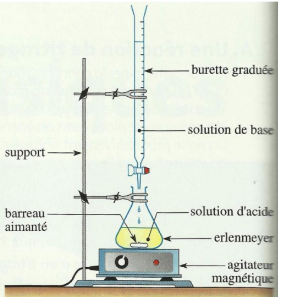
\includegraphics[width=0.3\textwidth]{./img/dosage00.png}
\end{wrapfigure}


On introduit dans un bécher un volume $V_A=20mL$ d'une solution d'acide éthanoïque $CH_3COOH$ de concentration $c_A$ inconnue puis
\\on lui ajoute progressivement à l'aide d'une burette graduée une solution d'hydroxyde de sodium $(Na^+ + HO^-)$ de concentration $c_B=0,02mol/L$.

On mesure le pH du mélange après chaque addition et on indique les valeurs obtenues dans le tableau suivant:


\begin{tabular}{|c|c|c|c|c|c|c|c|c|c|c|c|c|c|c|c|c|}
	\hline
	$V_B(mL)$ & 0& 2 &4&8&10&12&14&14,5&15&15,5&16&18&20&24&26&30\\\hline
	$pH$&2,9&3,4&3,6&3,9&4,1&4,5&5&5,8&7,6&10&11&11,3&11,4&11,5&11,6&11,7\\\hline
\end{tabular}
On trace la courbe représentant la variation du pH en fonction du volume VB de soude versé.

\begin{center}
	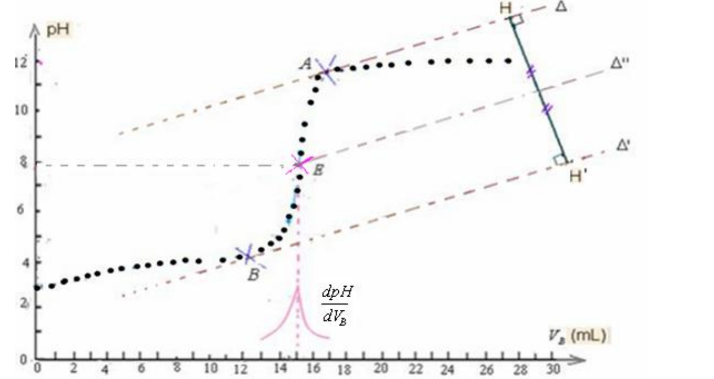
\includegraphics[width=0.5\textwidth]{./img/dosage01.png}
\end{center}

\subsection{Exploitation des résultats de l'expérience:}
\subsubsection{Equation de la réaction du dosage: }
Les ions $Na^+$ sont inactifs, ils ne participent pas à la réaction du dosage.

\ce{$CH_3COOH_{(aq)} + HO^-_{(aq)}$ -> $CH_3COO^-_{(aq)} + H_2O_{(l)} $}

C'est une réaction totale


\subsubsection{Détermination du point d'équivalence:}

\textbf{Méthode des tangentes : }On trace la droite $\Delta$ tangente à la courbe au point A et on trace la droite $\Delta$' parallèle à $\Delta$ au point
B, puis on représente le segment $[H,H']$ perpendiculaire à $\Delta$ et à $\Delta$'.
\\Ensuite on trace la droite $\Delta"$ médiatrice du segment $[H,H']$
.Cette dernière se coupe avec la courbe pH=f(VB) au point E.

Coordonnées du point d'équivalence E: $V_{BE}=15mL$ $pH_E = 7,8$


\textbf{Méthode de la courbe dérivée: } Cette méthode permet de déterminer le volume d'équivalence, elle consiste à tracer, à l'aide
d'un logiciel , la courbe dérivée: $\frac{dpH}{dV_B} = f(pH)$ Le volume d'équivalence VBE correspond à l'abscisse du maximum de cette courbe.

Cette méthode conduit dans le cas de notre dosage à $V_{BE}=15mL$.

\textbf{Méthode d’utilisation de l'indicateur coloré : }
Expérimentalement on détermine le volume d'équivalence en utilisant un
indicateur coloré ,lorsque sa couleur change brusquement à la teinte sensible on est à l'équivalence ,on obtient donc la valeur du
volume de soude versé à l'équivalence.

\underline{Choix de l'indicateur coloré: }L’indicateur coloré correspondant est celui dont la zone de virage contient le pH du point d'équivalence pHE.

Dans ce dosage le rouge de crésol est convenable car sa zone de virage:
$[7,2-8,8] $contient $pH_E = 7,8$.

\subsubsection{Relation d'équivalence: }

Avant l'équivalence, $HO^-$ est le réactif limitant ........Après l'équivalence, $CH_3COOH$ est le réactif limitant.

A l'équivalence le mélange est stœchiométrique : $n_i(CH_3COOH) = n_{eq}(HO^-)$

la relation d’équivalence est donc $C_A.V_A  = C_B.V_{BE}$
donc $C_A = \frac{C_B.V_{BE}}{V_A} = \frac{0,02.15.10^{-3}}{20.10^{-3}} = 1,5.10^{-2} mol/L$

\subsubsection{Détermination du taux d'avancement final de la réaction:}

Pour montrer que la réaction du dosage est totale, il suffit de montrer que:
$\tau = 1$.

Traçons le tableau d'avancement de la réaction au moment de versement du volume $V_{B}$versé=10mL de soude .

D'après la courbe du dosage le pH correspondant à ce volume est $pH=4,1$.

$n(CH_3COOH) = c_A.V_A = 0,015.0,02 = 3.10^{-4}mol = 0,3 mmol$


$n(OH^-) = c_B.V_B = 0,01.0,02 = 2.10^{-4}mol = 0,2 mmol$


\begin{tabular}{|c|c|c|c|c|c|}
	\hline
	\multicolumn{2}{|c|}{Equation de la réaction}& \multicolumn{4}{c|}{
\ce{CH_3COOH + HO^- ->[1][2] CH_3COO^- + H_2O}}\\\hline
	états  & avancement& \multicolumn{4}{|c|}{quantité de Matière en mmol}\\\hline
	Etat initial          &    0        &  0,3 &  0,2 &  0&  - \\\hline
				 \makecell{Etat de \\transformation}&$x$& 0,3-x & 0,2-x & $x$  & - \\\hline
				 Etat final            & $x_{eq}$ & $0,3 - x_{f}$ & $0,2 - x_{f}$  & $x_{f}$&- \\\hline
   % \cline{2-4}\
\end{tabular}

$HO^-$ est le réactif limitant et $x_{max}=0,2mmol$

A partir de l'état final qui correspond au $pH = 4,1$ et $[H_3O^+] = 10^{-4,1} mol/L$ 

le produit ionique de l'eau : $[H_3O^+].[HO^-] = 10^{-14}$ donc $[HO^-] = \frac{10^{-14}}{10^{-4,1}} = 10^{-9,9} mol/L$

alors $n_f(HO^-) = [HO^-].V_s = 10^{-9,9}.(10 + 20 ).10^{-3} = 3,10^{-11,9} = 3.10^{-8,9}mmol$

le taux d'avancement $\tau = \frac{x_f}{x_{max}} = \frac{0,2}{0,2} =1$


\section{Dosage d'une solution d'ammoniaque : }

\subsection{Etude expérimentale : }

On verse dans un bécher un volume $V_B=20mL$ d'une solution d'ammoniaque $NH_3$ de concentration $c_B$ inconnue puis on lui ajoute progressivement à l'aide d'une burette graduée une solution d'acide chlorhydrique
$(H_3O^+ + Cl^-)$ de concentration cA=1,2.10-2mol/L.


\begin{tabular}{|c|c|c|c|c|c|c|c|c|c|c|c|c|c|c|c|c|}
	\hline
	$V_B(mL)$ & 0& 1  &2 &3  &5  &7  &9&11 &13 &14 &14,5&15&16&17&18&20\\\hline
	$pH$    &10,6&10,3&10&9,8&9,5&9,2&9&8,7&8,2&7,3 &4,4&3,6&3,2&3&2,8&2,7\\\hline
\end{tabular}
On trace la courbe représentant la variation du pH en fonction du volume VB de soude versé.

\begin{center}
	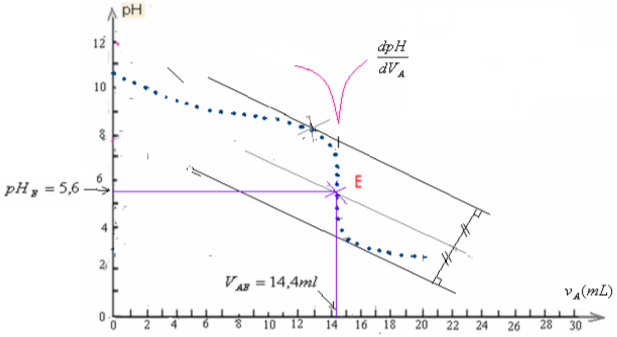
\includegraphics[width=0.8\textwidth]{./img/dosage03.png}
\end{center}


\subsection{Exploitation des résultats de l'expérience:}
\subsection{Equation de la réaction du dosage :}
Les ions $Cl^-$ sont inactifs, ils ne participent pas à la réaction du dosage. 

\ce{$NH_{3(aq)} + H_3O^+_{(aq)}$ -> $NH^+_{4(aq)} + H_2O_{(l)} $}

C'est une réaction totale


\subsubsection{Détermination du point d'équivalence:}
\textbf{La méthode des tangentes  }conduit à $pH_E = 5,6$ $V_{AE}=14,4mL$.
:
\\\textbf{La méthode de l'indicateur coloré:} D'après le tableau des indicateurs colorés on constate que c'est le rouge de méthyle
qui est convenable pour ce dosage , car sa zone de virage [4,2-6,2] contient le pHE=5,6.
\\\textbf{La méthode de la courbe dérivée }conduit dans ce cas à $V_{AE}=14,4mL$.


\subsubsection{Relation d'équivalence: }

Avant l'équivalence, $H_3O^+$ est le réactif limitant ........Après l'équivalence, $NH_3$ est le réactif limitant.

A l'équivalence le mélange est stœchiométrique : $n_i(NH_3H) = n_{eq}(H_3O^+)$

la relation d’équivalence est donc $C_A.V_A  = C_B.V_{BE}$
donc $C_B = \frac{C_A.V_{AE}}{V_B} = \frac{1,4.10^{-2}.14,4}{20} = 10^{-2} mol/L$

\begin{tcolorbox}
Remarque : Dans le cas du dosage d'une solution d'acide chlorhydrique $(H_3O^+ + Cl^-) $par une solution d'hydroxyde de sodium $(Na^+ + HO^-)$ ou bien l'inverse le pH du mélange à l'équivalence $pH_E = 7$
\end{tcolorbox}


%\subsection{Produit ionique de l'eau . }
%La réaction d'autoprotolyse de l'eau se produit dans toutes les solutions aqueuses.
%La constante d'équilibre associée à la réaction d'autoprotolyse de l'eau est :$$K_e = [H_3O^+]_{(eq)}.[HO^-]_{(eq)}$$

%Ke : s'appelle le produit ionique de l'eau.(il ne dépend que de la température).

%On utilise aussi le pKe qui est lié au produit ionique par la relation suivante:
%$K_e = 10^{-pKe}$ et $pKe$=$-log(Ke)$.


%Dans toutes les solutions aqueuses à $25^{\circ}C$ : $K_e = [H_3O^+].[HO^-]=10^{-14}$ donc $pKe = 14$

%\begin{center}
	%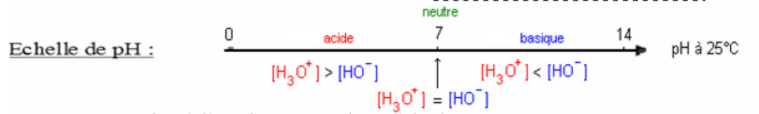
\includegraphics[width=0.7\textwidth]{./img/echellePH.png}
%\end{center}

%\section{Constante d'acidité d'un couple acide-base : }

%\subsection{Définition : }
%Pour un couple acide -base A/B , la réaction de l'acide A avec l'eau s'écrit: \ce{A + H_2O <=> B + H_3O^+}

%La constante d'acidité du couple acide-base A/B s'écrit: $K_A = \frac{[B][H_3O^+]}{[A]}$

%C'est une gradeur sans unité, qui ne dépend que de la température.

%On utilise aussi le pKA qui est lié à la constante d'acidité par la relation suivante:
%$K_A =  10^{-pKA}$ et $pKA = -log(K_A)$

%\subsection{Relation entre le pH et pKA: }
%D'après la relation de la constante d'acidité on a:$K_A = \frac{[B][H_3O^+]}{[A]}$ donc $[H_3O^+] = \frac{[A]K_A}{[B]} $

%aussi $pH = -log([H_3O^+])$ et $pH = -log(K_A) - log(\frac{[A]}{[B]})$

%alors $$pH = pKA + log(\frac{[B]}{[A]})$$


%\subsection{La constante d'équilibre K associée à une réaction acido-basique : }

%Pour le couple acide/base $A_1/B_1$ : \ce{A_1 + H_2O <=> B_1 + H_3O^+} la constante d'acidité $K_{A1}$=$\frac{[B_1][H_3O^+]}{[A_1]}$
%\\Pour le couple acide/base $A_2/B_2$ : \ce{A_2 + H_2O <=> B_2 + H_3O^+} la constante d'acidité $K_{A2}$=$\frac{[B_2][H_3O^+]}{[A_2]}$

%Dans la réaction acido-basique entre l'acide A1 du couple A1/B1 et la base B2 du couple A2/B2:

%\ce{A_1 + B_2 <=> A_2 + B_1} la constante d’équilibre $$K=\frac{[A_2][B_1]}{[A_1][B_2]} = \frac{K_{A1}}{K_{A2}} = 10^{pKA1 - pKA2}$$


%\section{Comparaison du comportement des acides et des bases : }
%\subsection{Comparaison des forces des acides : }
%\subsubsection{Influence du taux d'avancement final sur la force de l'acide : }
%Un acide $A_1H$ est plus fort qu'un acide $A_2H$, si, \underline{à concentrations égales}, le taux d'avancement de sa réaction avec l'eau
%est plus grand que celui de la réaction de l'acide $A_2H$ avec l'eau. $\tau_1\geq \tau_2 $).
%\\Pour des solutions de mêmes concentrations, l’acide le plus fort est celui dont le taux d’avancement final est le plus élevé.
%donc c’est celui pour lequel $[H_3O^+]$ est la plus élevée.

%$[H_3O^+]$ et $pH$ varient en sens inverses $(pH=-log[H_3O^+])$. 

%donc: l’acide le plus fort est celui pour lequel le pH est le plus faible

%\subsubsection{Influence de la constante d'acidité:}

%Tableau d'avancement de la réaction d'un acide A de concentration c , avec l'eau (volume de la solution V).:


%\begin{tabular}{|c|c|c|c|c|c|}
	%\hline
	%\multicolumn{2}{|c|}{Equation de la réaction}& \multicolumn{4}{c|}{
%\ce{A + H_2O <=>[1][2] B + H_3O^+}}\\\hline
	%états  & avancement& \multicolumn{4}{|c|}{quantité de Matière en mol}\\\hline
	%Etat initial          &    0        &  $n_i=C.V$ &  - &  0              &  0 \\\hline
				 %\makecell{Etat de \\transformation}&    $x$      & $C.V -x$ & - & $x$  & $x$ \\\hline
				 %Etat final            & $x_{eq}$ & $C.V - x_{eq}$ & -  & $x_{eq}$&$x_{eq}$ \\\hline
   %% \cline{2-4}\
%\end{tabular}

%L'eau est utilisée en excès, donc l'acide A est le réactif limitant. et Taux d'avancement à l'équilibre : $\tau = \frac{x_{eq}}{C.V}$.
%\\Avec $[H_3O^+] = [B] = \frac{x_{eq}}{V} = \frac{\tau.C.V}{V} = \tau.C$ et $[A] = \frac{C.V - X_{eq}}{V} = C(1-\tau)$
%\\La constante: d'acidité: $$K_A = \frac{[B][H_3O^+]}{[A]} = \frac{(C.\tau)^2}{C(1-\tau)} = \frac{C\tau^2}{1-\tau}$$

%\textbf{Un acide est d’autant plus fort que sa constante d’acidité KA est plus grande ou que son pKA est plus petit.}



%\subsection{Comparaison des forces des bases: }
%\subsubsection{Influence du taux d'avancement final sur la force de la base: }
%Une base B1 est plus forte qu’une base B2 ,si, à concentrations égales, le taux d’avancement de sa réaction avec l’eau
%est plus grand que celui de la réaction de la base B2 avec l’eau. ( $\tau_1>\tau_2$.)


%\subsubsection{Influence de la constante d'acidité: }
%Tableau d'avancement de la réaction de la base B de concentration c avec l'eau(volume de la solution V) .:


%\begin{tabular}{|c|c|c|c|c|c|}
	%\hline
	%\multicolumn{2}{|c|}{Equation de la réaction}& \multicolumn{4}{c|}{
%\ce{B + H_2O <=>[1][2] A + HO^-}}\\\hline
	%états  & avancement& \multicolumn{4}{|c|}{quantité de Matière en mol}\\\hline
	%Etat initial          &    0        &  $n_i=C.V$ &  - &  0              &  0 \\\hline
				 %\makecell{Etat de \\transformation}&    $x$      & $C.V -x$ & - & $x$  & $x$ \\\hline
				 %Etat final            & $x_{eq}$ & $C.V - x_{eq}$ & -  & $x_{eq}$&$x_{eq}$ \\\hline
   %% \cline{2-4}\
%\end{tabular}

%L'eau est utilisée en excès, donc La base B est le réactif limitant. et Taux d'avancement à l'équilibre : $\tau = \frac{x_{eq}}{C.V}$

%On a  $[B] = \frac{C.V-x_{eq}}{V} = C(1-\tau)$ et $[HO^-] = [A] = \frac{x_{eq}}{V} = C\tau$

%la constante d’équilibre associée à cette réaction : $$K = \frac{[A].[HO^-]}{[B]} = \frac{(C\tau)^2}{C(1-\tau)} = \frac{C\tau^2}{1-\tau}$$


%D'autre parte on a :	$K_A = \frac{[B].[H_3O^+]}{[A]} = \frac{Ke}{K} = \frac{1-\tau}{C.\tau}.Ke$


%\textbf{Une base est d’autant plus forte que la constante d’acidité KA associée au couple acide/base auquel elle appartient est plus petite
%ou que le pKA correspondant est plus grand.}

%\section{Diagramme de prédominance et celui de distribution : }

%\subsection{Diagramme de prédominance : }

%Relation liant le pH et le pKA est: $pH = pK_A + log(\frac{[B]}{[A]})$
%\\Si pH = pKA ; $log(\frac{[B]}{[A]}) = 0 $ donc $\frac{[B]}{[A]} = 1$ [B] = [A] acune des espèces A et B ne prédomine  
%\\Si $pH > pKA$ ; $log(\frac{[B]}{[A]}) > 0 $ donc $\frac{[B]}{[A]} > 1$ alors $[B] > [A]$ la base B prédomine  
%\\Si $pH < pKA$ ; $log(\frac{[B]}{[A]}) < 0 $ donc $\frac{[B]}{[A]} < 1$ alors $[B] < [A]$ l'acide A prédomine  

%Diagramme de prédominance:

%\begin{center}
	%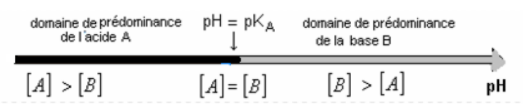
\includegraphics[width=0.5\textwidth]{./img/domainonace.png}
%\end{center}



%\subsection{Diagramme de répartition : }

%On considère une solution contenant l'acide A et sa base conjuguée B.
%\\On appelle pourcentage de l'acide A dans la solution, $\alpha(A) = \frac{[A]}{[A]+[B]}$
%\\On appelle pourcentage de la base B dans la solution, $\alpha(B) = \frac{[B]}{[A]+[B]}$
%\\Des logiciels de simulation permettent de donner les courbes représentant les pourcentages des espèces acide A et
%basique B d’un même couple dans une solution en fonction du pH de cette solution. On donne l’allure générale de
%cette distribution :.


%\begin{center}
	%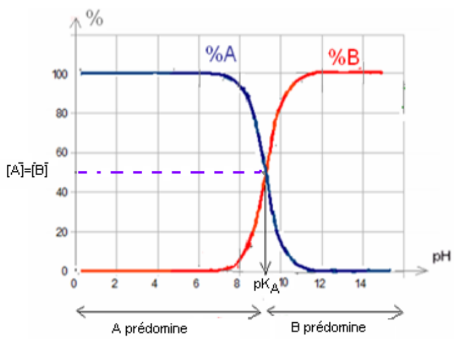
\includegraphics[width=0.5\textwidth]{./img/dominPH.png}
%\end{center}

%\subsection{Les Indicateur colorés : }
%Un indicateur coloré est un couple acide base $HIn/In^-$ ,dont les la forme acide HIn et la forme basique Inont des teintes différentes en solution aqueuse.
%\\Pour le bleu de bromothymol par exemple: la couleur de HIn est jaune et celle de $In^-$ est bleue.

%La forme acide HIn de l'indicateur réagit avec l'eau : \ce{HIn + H_2O <=> In^- + H_3O^+}


%Donc le pH de la solution est lié au pKA de l'indicateur coloré par la relation suivante :$pH = pKA + log({\frac{[In^-]}{[HIn]}})$


%\begin{itemize}
	%\item Lorsque la valeur du pH est voisine de celle du pKA , les deux formes HIn et Insont présentes avec des concentrations
%voisines , il y'a superposition des deux teintes et la couleur observée est dite teinte sensible.

%\item Généralement l'une des teintes prédomine et impose sa couleur si sa quantité est k fois supérieure à celle de l'autre.

%\item  la valeur de k dépend de l'indicateur , pour le (BBT) k=9 , c'est-à-dire si la concentration de HIn qui est jaune est 9 fois
%supérieure à celle de Inqui est bleu il prédomine et sa teinte apparait ) ceci qui entraine l'existence d'un intervalle de pH qui
%correspond à la teinte sensible qu'on appelle : la zone de virage.
%On donne dans le tableau suivant la zone de virage de quelques indicateurs colorés
%\end{itemize}

%\begin{center}
	%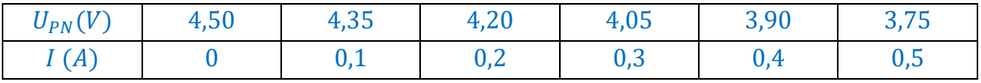
\includegraphics[width=0.5\textwidth]{./img/table.png}
%\end{center}



%\begin{figure}[h!]
	%\begin{center}
	%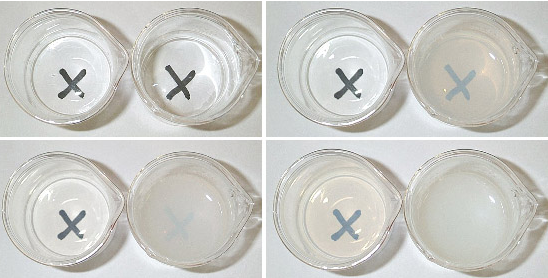
\includegraphics[width=0.5\textwidth]{./img/TRLconcentration.png}
%\end{center}
%\vspace{-1cm}
%\end{figure}



%\begin{wrapfigure}[10]{r}{0.5\textwidth}
%    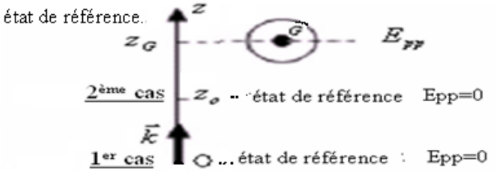
\includegraphics[width=0.5\textwidth]{./img/img00.png}
%\end{wrapfigure}


%\begin{center}
   %\begin{tabular}{|c|c|c|}
      %\hline
      %Indicateur coloré & Couleur de l’espèce acide & Couleur de l’espèce base\\\hline
      %BBT               & Jaune                     & Bleue\\\hline
      %Hélianthine       &Rose                       & Jaune\\\hline
      %Phénolphtaléine   & inclore                   & rose \\\hline
   %\end{tabular}
%\end{center}

\end{document}

